% Copyright (c) 2015-2021 Robert Ryszard Paciorek <rrp@opcode.eu.org>
% 
% MIT License
% 
% Permission is hereby granted, free of charge, to any person obtaining a copy
% of this software and associated documentation files (the "Software"), to deal
% in the Software without restriction, including without limitation the rights
% to use, copy, modify, merge, publish, distribute, sublicense, and/or sell
% copies of the Software, and to permit persons to whom the Software is
% furnished to do so, subject to the following conditions:
% 
% The above copyright notice and this permission notice shall be included in all
% copies or substantial portions of the Software.
% 
% THE SOFTWARE IS PROVIDED "AS IS", WITHOUT WARRANTY OF ANY KIND, EXPRESS OR
% IMPLIED, INCLUDING BUT NOT LIMITED TO THE WARRANTIES OF MERCHANTABILITY,
% FITNESS FOR A PARTICULAR PURPOSE AND NONINFRINGEMENT. IN NO EVENT SHALL THE
% AUTHORS OR COPYRIGHT HOLDERS BE LIABLE FOR ANY CLAIM, DAMAGES OR OTHER
% LIABILITY, WHETHER IN AN ACTION OF CONTRACT, TORT OR OTHERWISE, ARISING FROM,
% OUT OF OR IN CONNECTION WITH THE SOFTWARE OR THE USE OR OTHER DEALINGS IN THE
% SOFTWARE.

\section{Oświetlenie – podstawy fotometrii}

Jednym z istotnych zastosowań elektryczności jest oświetlanie.
Istnieje wiele parametrów związanych z tym jak jasno świeci dane źródło światła, czy też jak dobrze oświetlona jest dana powierzchnia.
Poniżej znajduje się krótkie wprowadzenie do tych zagadnień.

\subsection{Kąt bryłowy}

Kąt bryłowy wyrażany w steradianach [sr] jest to stosunek powierzchni wycinka kóli $S$ do jej promienia $r$: $$\Omega = S / r^2 \quad [{\rm sr}]$$
Taki wycinek kóli może zostać utworzony poprzez obrót wokół jednego z boków wycinka koła o promieniu $r$ i kącie pomiędzy dwoma promieniami wynoszącym $\alpha$.

\begin{center}
	\begin{minipage}{1.5cm}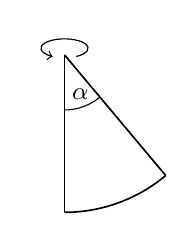
\begin{tikzpicture}[semithick]
		\node[yshift=1mm] {
			\tikz [x=0.12cm,y=0.30cm,line width=.1ex,->,rotate=90] \draw (0,0) arc (-150:150:1 and 1);
		};
		\draw[thin] (0,0) -- ++(270:2cm);
		\draw (0,0) -- ++(310:2cm);
		\draw ([shift=(270:2cm)]0,0) arc (270:310:2cm);
		
		\node[yshift=-5mm,xshift=2mm] {\small$\alpha$};
		\draw[thin] ([shift=(270:7mm)]0,0) arc (270:310:7mm);
	\end{tikzpicture}
	\end{minipage}
	\hspace{0.9cm}$\Rightarrow$\hspace{0.9cm}
	\begin{minipage}{3cm}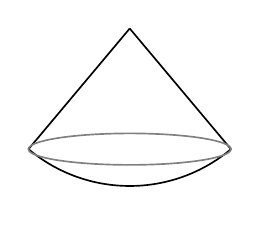
\begin{tikzpicture}[semithick]
		\draw (0,0) -- ++(230:2cm);
		\draw (0,0) -- ++(310:2cm);
		\draw ([shift=(230:2cm)]0,0) arc (230:310:2cm);.
		\draw[gray] ([yshift=-2cm * cos{40}]0,0)ellipse (2cm * sin{40} and 0.2cm);
	\end{tikzpicture}
	\end{minipage}
\end{center}

wtedy: $$\Omega = 2 \pi (1 - \cos (\alpha)) \qquad \Omega \in [0, 4\pi] \Leftrightarrow \Omega \in [0, 12.56\ldots]$$

W przekroju wtedy taki wycinek kóli posiada kąt rozwarcia (który jest także kątem rozwarcia stożka, o tej samej powierzchni stożkowej co ten wycinek kóli): $$\theta = 2 \alpha$$


\subsection{Charakterystyka źródła światła}

\subsubsection{strumień świetlny [lumen, lm]}

Podstawowym parametrem charakteryzującym źródło światła jest emitowany strumień świetlny $\Phi$, którego wartość wyrażana jest w lumenach [lm].

\subsubsection{kąt świecenia}

Drugim parametrem opisującym źródło światła jest kąt bryłowy $\Omega$, w którym emituje ono generowany przez siebie strumień świetlny\footnote{dla uproszenia będziemy zakładać że źródło w całym tym kącie bryłowym emituje promieniowanie równomiernie}.

Kąt świecenia podawany jest jednak zazwyczaj jako kąt rozwarcia stożka świecenia $\theta$, a rzadziej jako kąt bryłowy $\Omega$.
Wiemy jednak że: $\Omega = 2 \pi (1 - \cos (\theta/2))$.

\subsubsection{natężenie strumienia świetlnego [kandela, cd]}

Te dwie wartości pozwalają na obliczenie \strong{światłości} (natężenia strumienia świetlnego) $I$, wyrażanej w kandelach \strong{[cd]}.
$$I = {\Phi \over \Omega} = {\Phi \over 2 \pi (1 - \cos (\theta/2))} \quad \left[{\rm {lm \over sr} = cd}\right]$$

W im większy kąt źródło o danym strumieniu będzie świecić, tym natężenie tego strumienia będzie mniejsze.
Minimum osiągnie dla punktowego źródła izotropowego (świecącego tak samo w każdym kierunku), dla którego:
	$I = {\Phi \over 4 \pi}$ (co odpowiada stożkowi o kącie rozwarcia $\theta = 2 \pi$).


\subsection{Charakterystyka oświetlenia}

W codziennych zastosowaniach zazwyczaj bardziej interesuje nas jasność oświetlenia jakieś powierzchni oddalonej o $r$ od źródła światła niż jasność samego źródła światła.

\subsubsection{natężenie oświetlenia [luks, lx]}

Do określenia jak dobrze oświetlona jest dana powierzchnia stosowane jest natężenie oświetlenia $E$ wyrażane w luksach [lx].
Przy założeniu prostopadłego padania światła na powierzchnię $S$ (czyli np. dla wycinka kóli o promieniu $r$ z źródłem światła w środku):
	$$E = {\Phi \over S} \quad \left[{\rm {lm \over m^2} = lx}\right]$$
Taki wycinek kóli odpowiada kątowi bryłowemu $\Omega = S/r^2$ (z definicji kąta bryłowego), czyli:
	$$E = {\Phi \over \Omega r^2} = {I \over r^2}$$


\subsection{Przykłady źródeł światła}

\subsubsection{świetlówka T8}
$$83 \dots 96 lm/W \qquad\Rightarrow\qquad 6.61 \dots 7.67 cd/W$$

\subsubsection{dioda LED biała 3W}
$$140^\circ, 100lm \quad\Rightarrow\quad \alpha = 70^\circ \quad\Rightarrow\quad$$
$$\Omega = 2 \pi (1 - \cos (70\pi/180)) = 4.134 \rm sr \quad\Rightarrow\quad  24cd \quad\Rightarrow\quad 8 cd/W$$
